\chapter{Projet effectué}

Dans ce chapitre, je détaillerai le projet auquel j'ai contribué lors de mon stage au sein de l'équipe de développement de. Ce projet avait pour objectif la conception et la mise en œuvre d'une solution numérique innovante. L'intégration de nouvelles technologies a joué un rôle clé dans la réussite de cette initiative.

\section{Conception du Projet}

La phase de conception du projet a été déterminante pour définir l'architecture globale et les fonctionnalités principales du système. Nous avons pris des décisions importantes concernant la structure de la base de données, la répartition des rôles, ainsi que les choix techniques en matière de développement. L'utilisation de méthodologies agiles a permis de structurer les différentes étapes du projet tout en assurant une flexibilité dans les ajustements en cours de route.

\subsection{Modélisation des Cas d'Utilisation}

La modélisation des cas d'utilisation a permis d'identifier les principaux acteurs et leurs interactions avec le système. Le diagramme de cas d'utilisation ci-dessous présente les interactions essentielles. L'acteur principal, "Utilisateur", est capable d'interagir avec l'application pour effectuer des tâches variées telles que la gestion des ressources, l'accès aux données ou la création de nouveaux objets dans le système. Chaque cas d'utilisation a été minutieusement analysé pour garantir que les fonctionnalités répondent aux besoins des utilisateurs finaux.\\
La modélisation des cas d'utilisation a permis d'identifier les principaux acteurs et leurs interactions avec le système. Le diagramme de cas d'utilisation ci-dessous présente les interactions essentielles. L'acteur principal, "Utilisateur", est capable d'interagir avec l'application pour effectuer des tâches variées telles que la gestion des ressources, l'accès aux données ou la création de nouveaux objets dans le système. Chaque cas d'utilisation a été minutieusement analysé pour garantir que les fonctionnalités répondent aux besoins des utilisateurs finaux.
\clearpage
%%%%%%%%%%%%%%%%%%%%%%%%%%%%%%%%%%%%%%%%%%%%%%%%%%%%%%%%%%%%%%%%%%%%%
% Best thing to do if the pictures are begin acting weard just   add %two pics in the same page then \clearpage that my help you
%%%%%%%%%%%%%%%%%%%%%%%%%%%%%%%%%%%%%%%%%%%%%%%%%%%%%%%%%%%%%%%%%%%%%% 
\section{Les interfaces de l'application}
\subsection{Partie Web}
Pour avoir accès aux différentes fonctionnalités de l'application, il faut se connecter. Si l'authentification échoue, le formulaire affiche un message d'erreur. 
\begin{figure}[hbt!]
	\centering
	\fbox{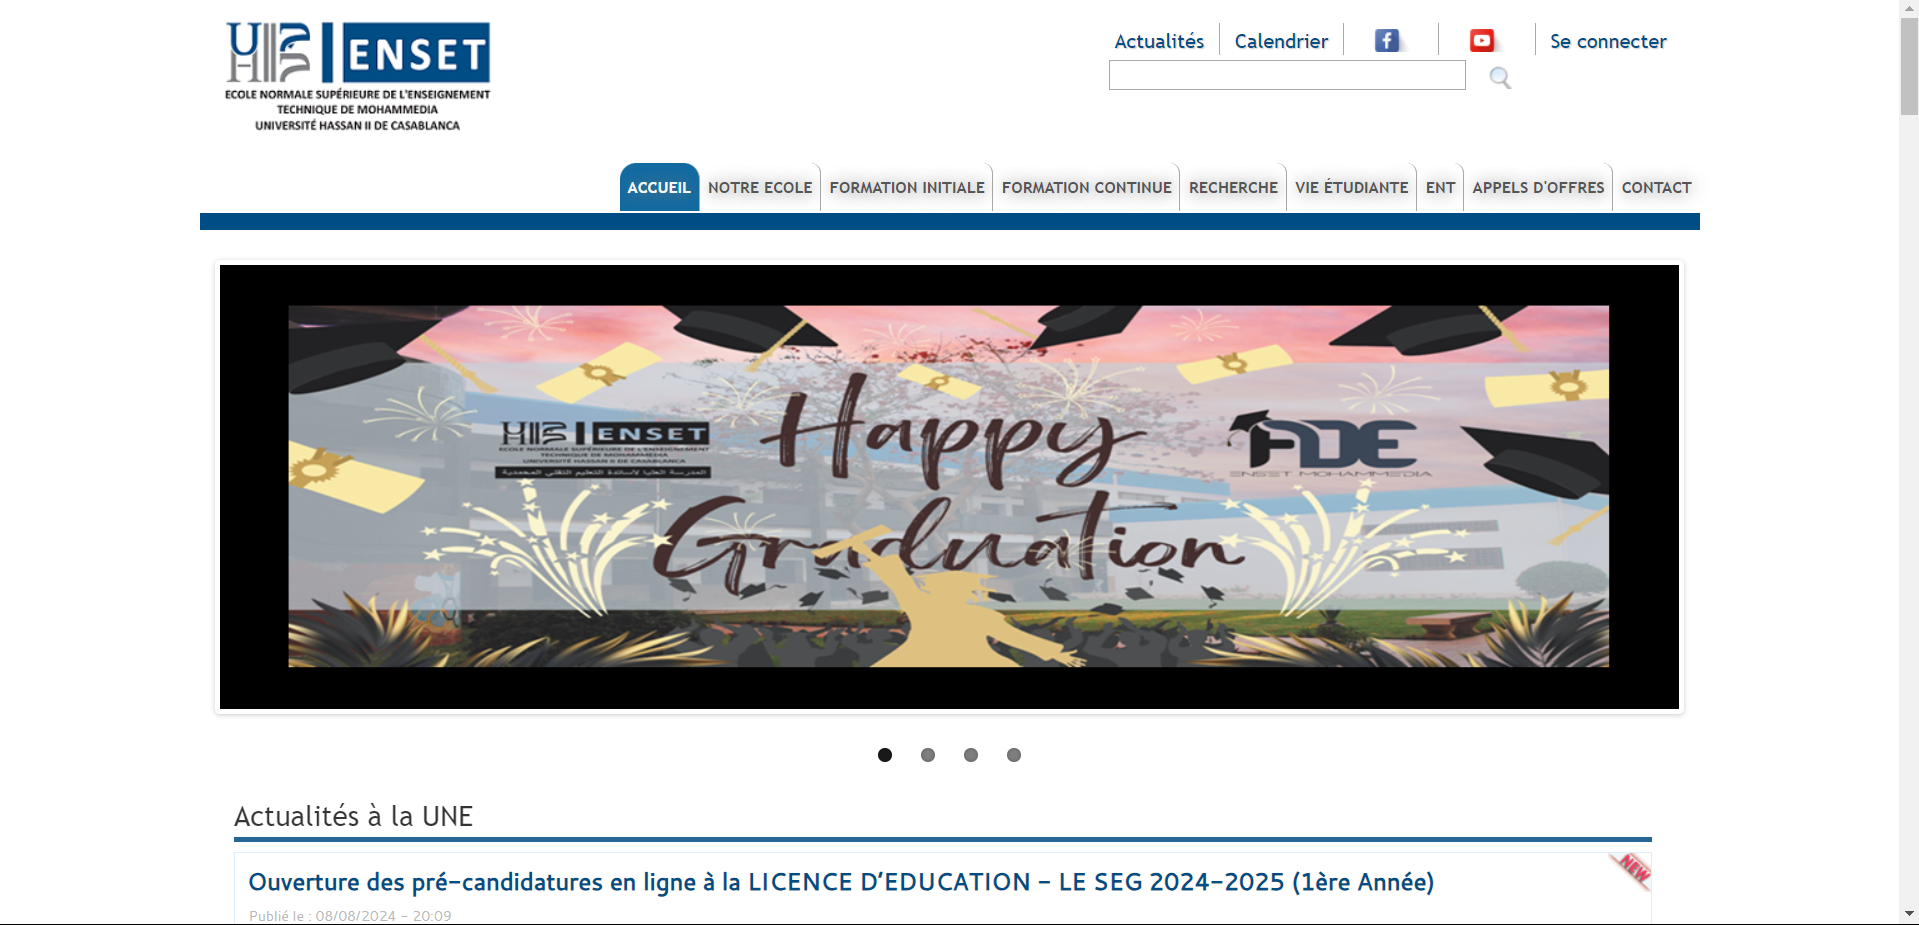
\includegraphics[width=15cm]{screens/Screenshot 2024-08-22 212533.png}}
	\caption{Page d'authentification vers la plate-forme.}
	\label{fig:1}
\end{figure}
\newline

\begin{figure}[hbt!]
	\centering
	\fbox{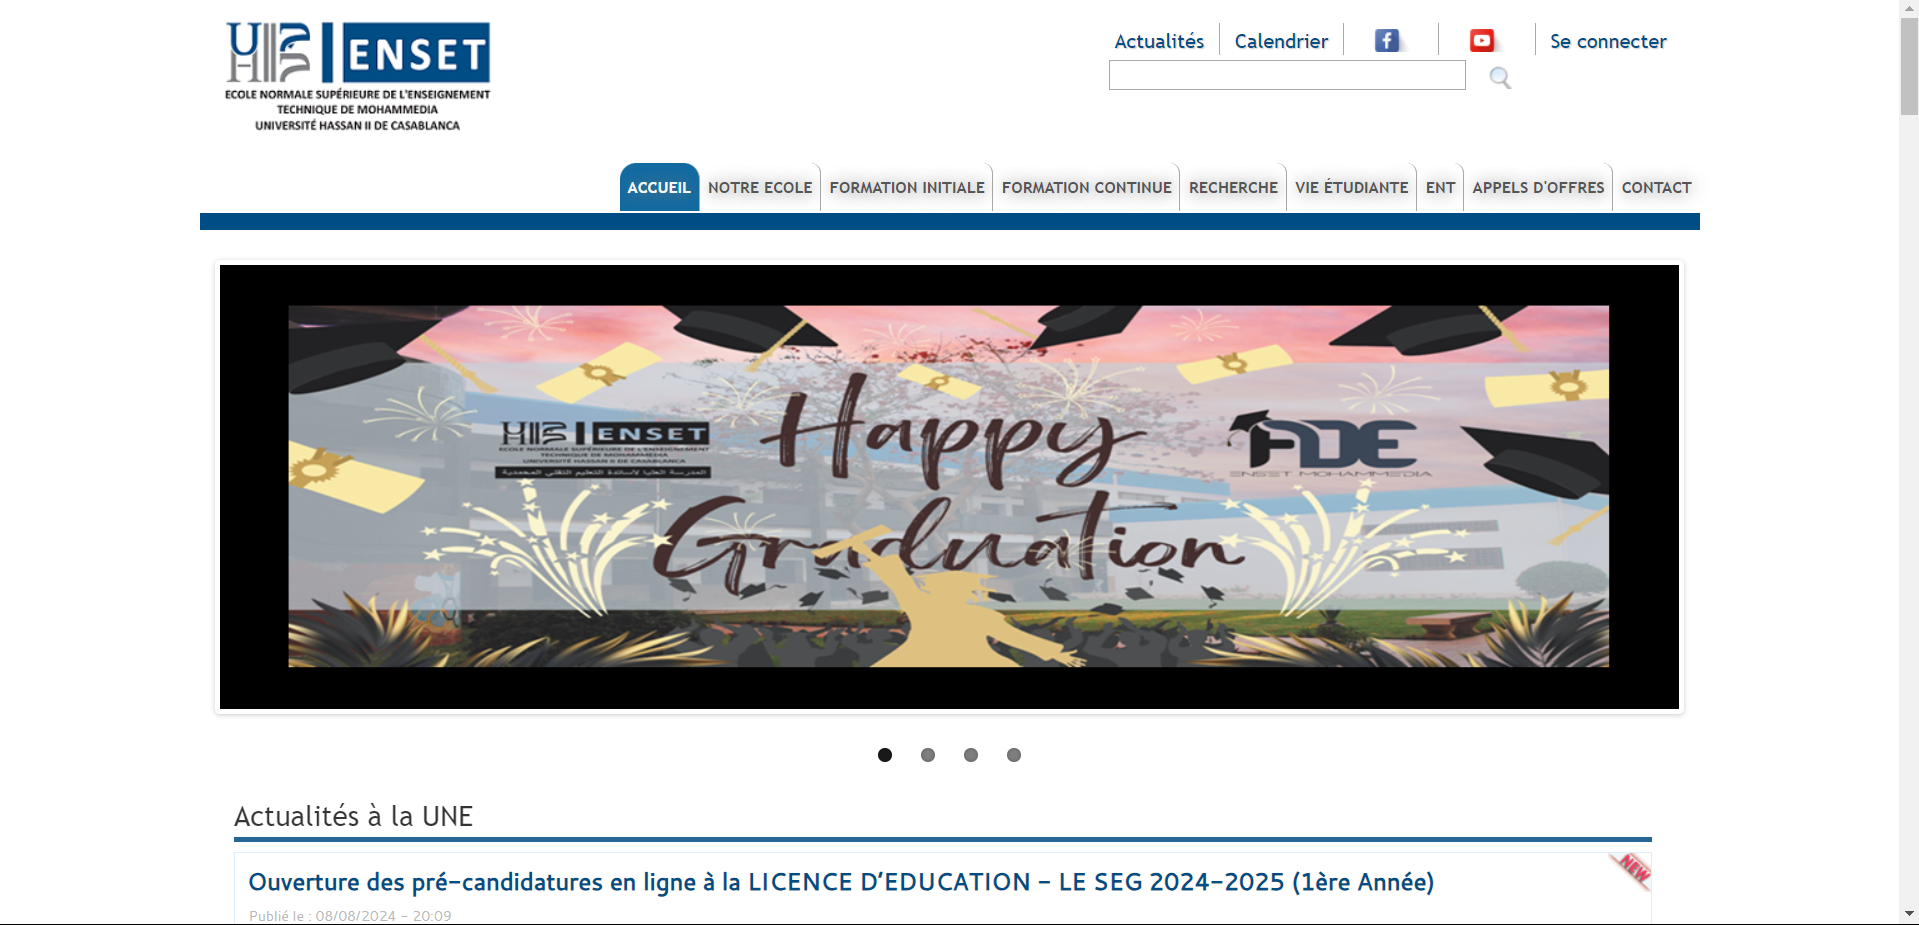
\includegraphics[width=15cm]{screens/Screenshot 2024-08-22 212533.png}}
	\caption{Accueil.}
	\label{fig:1}
\end{figure}
La page d'accueil présente le logo ainsi qu'une courte description.
\clearpage
%%%%%%%%%%%%%%%%%%%%%%%%%%%%%%%%%%%%%%%%%%%%%%%%%%%%%%%%%%%%%%%

\subsection{Partie Mobile}

\begin{figure}[ht]
  \centering
  \begin{minipage}{0.45\textwidth}
    \vspace{0.5cm}% Ajuster l'espace vertical si nécessaire
    La page de connexion affiche le logo de la page et un formulaire d'authentification demandant l'adresse e-mail et le mot de passe pour se connecter et accéder à l'écran d'accueil.
  \end{minipage}%
  \hspace{0.05\textwidth}% Ajuster l'espace horizontal si nécessaire
  \begin{minipage}{0.5\textwidth}
    \centering
    \fbox{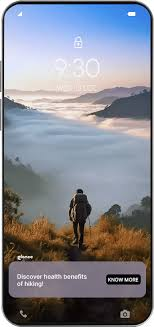
\includegraphics{Mobile/images.jpeg}}
    \caption{Page de connexion}
    \label{fig:login_page}
  \end{minipage}
\end{figure}

\section{Conclusion}
La modélisation des cas d'utilisation a permis d'identifier les principaux acteurs et leurs interactions avec le système. Le diagramme de cas d'utilisation ci-dessous présente les interactions essentielles.